%%%%%%%%%%%%%%%%%%%%%%% file template.tex %%%%%%%%%%%%%%%%%%%%%%%%%
%
% This is a general template file for the LaTeX package SVJour3
% for Springer journals.          Springer Heidelberg 2010/09/16
%
% Copy it to a new file with a new name and use it as the basis
% for your article. Delete % signs as needed.
%
% This template includes a few options for different layouts and
% content for various journals. Please consult a previous issue of
% your journal as needed.
%
%%%%%%%%%%%%%%%%%%%%%%%%%%%%%%%%%%%%%%%%%%%%%%%%%%%%%%%%%%%%%%%%%%%
%
% First comes an example EPS file -- just ignore it and
% proceed on the \documentclass line
% your LaTeX will extract the file if required
\begin{filecontents*}{example.eps}
%!PS-Adobe-3.0 EPSF-3.0
%%BoundingBox: 19 19 221 221
%%CreationDate: Mon Sep 29 1997
%%Creator: programmed by hand (JK)
%%EndComments
gsave
newpath
  20 20 moveto
  20 220 lineto
  220 220 lineto
  220 20 lineto
closepath
2 setlinewidth
gsave
  .4 setgray fill
grestore
stroke
grestore
\end{filecontents*}
%
\RequirePackage{fix-cm}
%
%\documentclass{svjour3}                     % onecolumn (standard format)
%\documentclass[smallcondensed]{svjour3}     % onecolumn (ditto)
\documentclass[smallextended]{svjour3}       % onecolumn (second format)
%\documentclass[twocolumn]{svjour3}          % twocolumn
%
\smartqed  % flush right qed marks, e.g. at end of proof
%
%
% \usepackage{mathptmx}      % use Times fonts if available on your TeX system
%
% insert here the call for the packages your document requires
%\usepackage{latexsym}
%\usepackage{longtable}

\usepackage{xfrac}   
\usepackage{lineno}  
\usepackage{graphicx}
\usepackage{color}
\usepackage{multirow}
\usepackage{array}
\usepackage{setspace} 
\usepackage{makecell}
\usepackage[nomarkers]{endfloat}

%DEFINED BY NELSON NAZZICARI: defining this command so we can have 
% wrapping (p) columns horizontally centered in tables
\newcolumntype{C}[1]{>{\centering\let\newline\\\arraybackslash\hspace{0pt}}m{#1}}

%ADDED FOR PEER REVIEW: these commands to be deleted in the final version
\linenumbers
\doublespacing %this command to be removed

% Insert the name of "your journal" with
\journalname{Molecular Breeding}
%
\begin{document}

\title{
Marker imputation efficiency for Genotyping-By-Sequencing data in rice (\emph{Oryza sativa}) and alfalfa (\emph{Medicago sativa})
\thanks{Nelson Nazzicari and Filippo Biscarini contributed equally to the work \\
Corresponding author: Nelson Nazzicari \email{nelson.nazzicari@entecra.it}}
}
%\subtitle{Do you have a subtitle?\\ If so, write it here}

% if too long for running head
\titlerunning{Imputation efficiency for GBS data with and without the reference genome}        

\author{Nelson Nazzicari \and
  Filippo Biscarini  \and
  Paolo Cozzi \and
  E. Charles Brummer \and
  Paolo Annicchiarico
}

\authorrunning{Nazzicari, Biscarini et al.} % if too long for running head

\institute{
    N. Nazzicari, P. Annicchiarico \at Council for Agricultural Research and Economics (CRA) Research Centre for Fodder Crops and Dairy Productions, Lodi (Italy)
\and
    F. Biscarini, P. Cozzi \at Dipartimento di Bioinformatica, Fondazione Parco Tecnologico Padano, Lodi (Italy)
\and
    E.C. Brummer \at University of California, Plant Sciences Department, Davis, CA (USA)
}


\date{Received:  / Accepted:}
% The correct dates will be entered by the editor

\maketitle

\graphicspath{{./figures/}}
\begin{abstract}
Genotyping-by-sequencing (GBS) is a rapid and cost-effective genome-wide 
genotyping technique applicable whether a reference genome is available 
or not. Due to the cost-coverage trade-off, however, GBS typically produces 
large amounts of missing marker genotypes, whose imputation becomes therefore 
both challenging and critical for later analyses.\\
In this work, the performance of four general imputation methods (K-Nearest 
Neighbors, Random Forest, Singular Value Decomposition, and Mean Value)
and two genotype-specific methods (``Beagle'' and FILLIN) were measured 
on GBS data from alfalfa (\emph{Medicago sativa L.}, autotetraploid, heterozygous, 
without reference genome) and 
rice (\emph{Oryza sativa L.}, diploid, 100\% homozygous, with reference genome). Alfalfa SNP were aligned on the genome of the closely related species \emph{Medicago truncatula L.}. Benchmarks 
consisted in progressive data filtering for marker call-rate (up to 70\%) and increasing 
proportions (up to 20\%) of known genotypes masked for imputation. The 
relative performance was measured as the total proportion of correctly imputed 
genotypes, globally and within each genotype class (two homozygotes in rice, 
two homozygotes and one heterozygote in alfalfa).\\
We found that imputation accuracy was robust to increasing 
missing rates, and consistently higher in rice than in alfalfa. Accuracy 
was as high as 90-100\% for the major (most frequent) homozygous genotype, but dropped 
to 80-90\% (rice) and below 30\% (alfalfa) in the minor homozygous genotype. 
Beagle was the best performing method, both accuracy- 
and time-wise, in rice. In alfalfa, KNNI and RFI gave the highest accuracies, but KNNI 
was much faster.

\keywords{SNP, Genotyping by Sequencing (GBS), K-Nearest Neighbors Imputation 
(KNNI), Random Forest Imputation (RFI), Singular Value Decomposition Imputation 
(SVDI), Beagle, FILLIN, alfalfa, rice, imputation, reference genome}
\end{abstract}




\section{Introduction}
\label{intro}

Imputation of missing alleles and genotypes is usually a preliminary step for
a wide range of genetic analyses: in fact, most models and software for 
population genetics, genomic selection (GS) and genome-wide association 
studies (GWAS) can not handle missing data and require complete datasets. 
SNP-chips represent one of the leading genotyping technologies, and produce 
datasets that, after markers and individuals with low call-rate are edited out, 
usually still contain a small proportion of uncalled genotypes (e.g., $<$5\%) 
randomly distributed along the genome. Genotyping-by-sequencing (GBS) is a 
relatively recent genotyping technique alternative to SNP-chips that can 
be used to produce SNP genotype data~\cite{elshire_robust_2011}.
GBS is platform-independent and is conveniently 
used in species that lack commercial SNP-chips or even lack a reference 
genome sequence. GBS data typically present a much larger proportion of 
sporadic missing genotypes: e.g., $\sim$52\% average in maize \cite{crossa_genomic_2013},
or up to 80\% for a fraction of SNPs in wheat \cite{poland_genomic_2012}. This 
is due to both intrinsic properties of the technology - e.g., low coverage - 
and to its application to species without a mature genome assembly \cite{glaubitz_tassel-gbs:_2014}.\\
There are several methods that are routinely used for the imputation of 
missing genotypes. Some rely solely on genotypic information, some make 
use also of genealogies, most of them are based on reconstructing haplotypes 
to be used in predictive models \cite{nicolazzi_software_2015}. Most methods for 
genotype imputation have been developed for SNP-chip data, and typically 
yield very high imputation accuracy: for instance, $>$95\% correctly imputed 
genotypes were reported in maize \cite{hickey_factors_2012} and cattle \cite{vanraden_genomic_2011}. 
Such methods can be applied to GBS data, too (see for instance 
\cite{huang_efficient_2014} and \cite{swarts_novel_2014} 
for applications in rice and maize). When a reference 
genome is available, SNP loci can be aligned against its sequence and 
are therefore ordered. However, GBS data may be generated 
also for species lacking a reference genome assembly. In this case the 
GBS output is a series of ``floating'' loci not linked to any chromosome: 
alignment is not possible and SNPs are therefore unordered. Unordered 
data add additional complexity to the task of imputing missing genotypes: 
exploitation of linkage disequilibrium (LD) and haplotype reconstruction 
are less straightforward, consecutive loci may lie on different chromosomes
or scaffolds, and overall data are less homogeneous. Rutkoski et al.~\cite{rutkoski_imputation_2013}
considered the application of general data imputation methods 
to wheat, maize and barley populations, obtaining best case scenarios accuracies 
as high as 0.84-0.94 (measured as $R^{2}$ between true and imputed genotypes).\\
Compared to SNP-chip data, GBS data are more challenging: many more 
missing genotypes, high variability between runs, intrinsically noisy data, 
reads from different loci that can overlap. For all these reasons, imputation 
of missing genotypes with GBS data is still a relatively immature technique, 
not yet amenable to produce highly standardised and repeatable results. 
There is therefore scientific and practical interest in gaining further 
insights into how genotype imputation with GBS data works, and in 
developing the best methods and strategies to accurately and efficiently 
impute such missing data. This would be relevant not only for the scientific 
community but also for the breeding industry, because of its direct 
consequences on genomic applications.\\
In this paper, we imputed missing genotypes from GBS data in two agronomically
important crop species: the forage crop alfalfa (\emph{Medicago sativa}), for 
which a reference genome is not available yet, and the 
cereal crop rice (\emph{Oryza sativa}) whose reference genome has been 
assembled \cite{international_rice_genome_sequencing_project_map-based_2005} and
recently updated \cite{kawahara_improvement_2013}. We compared the imputation 
efficiency of four general data-imputation methods (Mean Value Imputation, 
K-Nearest Neighbour Imputation, Singular Value Decomposition Imputation 
and Random Forest Imputation) with the performance of two methods specific 
for genotype imputation (localized haplotype clustering imputation, 
implemented in the software package Beagle, %and haplotype reconstruction around the recombination site
and the FILLIN algorithm implemented in the programming suite Tassel). The relative efficiency of 
the different imputation methods was assessed in terms of the 
accuracy achieved and the computation time required. Not only the total imputation accuracy was measured, but also the accuracy of imputing the different genotype classes (major and minor homozygotes, heterozygotes).\\

\section{Materials and methods}

\subsection{Plant material}
\label{sec:plant_material}

Samples from two autotetraploid alfalfa (\emph{Medicago sativa L.}) and one diploid rice (\emph{Oryza sativa L.}) populations were available (see Table~\ref{tab:descriptive_statistics}).\\
Alfalfa populations included elite germplasms from the Po Valley (Alfalfa-PV) and Mediterranean-climate environments (Alfalfa-Med). For Alfalfa-PV, 124 parent genotypes were chosen by stratified mass selection for dry matter yield over three harvests. For Alfalfa-Med, 154 parent genotypes were derived from two cycles of free intercrossing among three outstanding populations in a multi-environment study. For further details see \cite{Annicchiarico2015}. \\
The Rice dataset included 437 plants belonging to 391 accessions (46 duplicates) from the Rice Germplasm Collection maintained at CRA-Rice Research Unit (Vercelli, Italy). The sampled collection comprised accessions from the five main sub-populations of \emph{O. sativa} (274 temperate japonica, 108 tropical japonica, 28 indica, 16 aus and 11 aromatic). All accessions were purified through single seed descent, and were genotypically essentially 100\% homozygous.

\subsection{Genotyping by sequencing}
\label{sec:overview}

The 715 samples from alfalfa (Alfalfa-Med and Alfalfa-PV) and rice (Rice) populations were genotyped using the genotyping-by-sequencing (GBS) approach \cite{elshire_robust_2011}. Different GBS protocols were used to genotype the alfalfa and rice samples, since genotyping was carried out under different projects.\\
In alfalfa, DNA was isolated from fresh leaf tissues by the Wizard~\textregistered~Genomic DNA Purification Kit (Promega, A1125) and quantified with a Quant-iT PicoGreen dsDNA assay kit (Life Technologies, P7589). Two libraries were constructed for the two populations, where 100 ng of each DNA was digested with ApeKI (NEB, R0643L) and then ligated to a unique barcoded adapter and a common adapter. For the reference population Alfalfa-Med, 5 nmoles each of the primers and NEB 2X Taq Master Mix (NEB Cat \# M0270S) were included in the PCR reaction according to \cite{elshire_robust_2011} original protocol, while for Alfalfa-PV the KAPA library amplification readymix (Kapa Biosystems Cat \# KK2611) was used instead. Each library was sequenced in two lanes on Illumina HiSeq 2000 at the Genomic Sequencing and Analysis Facility at the University of Texas at Austin, Texas, USA. For both populations post sequencing analysis and SNP calling was carried out using Tassel UNEAK pipeline \cite{lu_switchgrass_2013}.

Alfalfa is an autotetraploid plant species and can therefore present three different heterozygous genotypes: AAAB, AABB and ABBB. Sequencing depth in this study was not sufficient for accurate tetraploid allelic dosage, but following \cite{li_saturated_2014} and \cite{li_genomic_2015} reliable genotype calls based on diploid allelic dosage were obtained considering diploid heterozygotes (i.e. AB), while the two homozygous genotypes (AAAA and BBBB) were considered diploid homozygotes (i.e., AA or BB). A further quality filter, implemented through ad-hoc Python scripts, removed heterozygous loci with less than 4 and homozygous loci with less than 11 aligned reads. A similar filtering was performed in \cite{Rocher_validation_2015} using less restrictive thresholds. 

In rice, DNA was isolated from three-weeks old leaves using the DNeasy Plant Mini Kit (QIAGEN) with a TECAN Freedom EVO150 liquid handling robot (TECAN Group Ltd, Switzerland). DNA digestion was performed on 100 ng samples in 96-well plates using ApeKI, which was shown to cut every 1 kb on average in a in-silico digestion of the Nipponbare reference genome, and 96-plex libraries constructed according to the GBS protocol. The libraries were loaded into Genome Analyzer II (Illumina, Inc., San Diego, CA) for sequencing. Raw sequence data filtering, sequence alignment to the rice reference genome (Os-Nipponbare-Reference-IRGSP-1.0, \cite{kawahara_improvement_2013}), and SNP calling from GBS genotyping were carried out using the Tassel GBS pipeline \cite{glaubitz_tassel-gbs:_2014}.\\
In total, 32\,706, 40\,734 and 166\,418 SNP markers were called by GBS in Alfalfa-PV, Alfalfa-Med and Rice, respectively (see Table~\ref{tab:descriptive_statistics}). In all datasets SNP variants were renamed so that AA represented the most common homozygote, and BB the least common homozygote.

\begin{table}
\centering
\caption[Descriptive statistics]{
Descriptive statistics of alfalfa (\emph{Medicago sativa L.}) 
and rice (\emph{Oryza sativa L.}) genotyping. MAF is average minor allele frequency; 
p(AA), p(AB) and p(BB) are the proportions of AA, AB and BB genotypes.}
\label{tab:descriptive_statistics}
\begin{tabular}{lccccccc}
\hline\noalign{\smallskip}
\noalign{\smallskip}\hline\noalign{\smallskip}
\textbf{Dataset} & \textbf{No. samples} & \textbf{No. SNPs} & \textbf{Missing Rate} & \textbf{MAF} & \textbf{p(AA)} & \textbf{p(AB)} & \textbf{p(BB)}\\
\noalign{\smallskip}\Xhline{3\arrayrulewidth}\noalign{\smallskip}
Alfalfa-PV & 124 & 32\,706 & 0.666 & 0.1724 & 0.690 & 0.274 & 0.035\\
Alfalfa-Med & 154 & 40\,734 & 0.596 & 0.1702 & 0.691 & 0.276 & 0.032\\
Rice & 437 & 166\,418 & 0.534 & 0.140 & 0.860 & - & 0.140 \\
\noalign{\smallskip}\hline
\end{tabular}
\end{table}


\subsection{Imputation methods}
\label{sec:imputation_methods}
We considered six imputation methods: Mean Value Imputation (MNI), K-Nearest Neighbors Imputation (KNNI), Random Forest Imputation (RFI), Singular Value Decomposition Imputation (SVDI), Localized Haplotype Clustering Imputation (``Beagle'') and haplotype reconstruction around the recombination sites (FILLIN from Tassel suite). For all algorithms we imputed a $m\times n$ matrix of m individuals and n markers whose data points, defined in the set \{0,1,2,NA\}, represented the three possible genotypes (AA, AB, and BB) and the missing value, respectively. 
\paragraph{MNI}
\label{par:MNI}
: in Mean Value Imputation each missing data point was replaced by the mean of the non-missing values for that marker, then discretized to the closest value in \{0,1,2\}.
\paragraph{KNNI}
\label{par:KNNI}
: in K-Nearest Neighbors Imputation missing data points were imputed based on the weighted average of the K closest markers \cite{troyanskaya_missing_2001} defined by the Simple Matching Coefficient distance function \cite{schwender_statistical_2007}, specifically designed for categorical data. $K=4$ was used in KNNI, and neighbo
rs values were weighted by the reciprocal of their distance from the data point to be imputed.
\paragraph{SVDI}
\label{par:SVDI}
: Singular Value Decomposition (SVD) imputation was based on the following factorization of the genotype matrix M (m markers, n individuals):

\begin{equation}
\label{eq:SVDI_general}
M = U\Sigma V^{T}
\end{equation}

where U is a $m \times m$ unitary matrix (i.e. $UU^{T}=I$), $\Sigma$ is a $m \times n$ rectangular diagonal matrix of singular values and $V^{T}$ is the $n \times n$ conjugate transpose of the unitary matrix V. Matrix U and V contain the eigenvectors of $M^{T}M$ and $MM^{T}$, respectively, and the corresponding non-zero singular values in $\Sigma$ are equivalent to the square-root of the eigenvalues of $M^{T}M$ and $MM^{T}$. The first k eigenvectors - ordered by decreasing eigenvalue - capture most of the information in the marker genotype matrix, and were used to generate linear combinations (principal components) of the original m markers for the imputation of missing data points. The imputation procedure comprised: (i) initial imputation of missing genotypes using MNI, since SVD can only be performed on complete matrices; (ii) SVD to select the most informative k eigenvectors of the marker genotype matrix; (iii) these k eigenvectors were used as predictors in a linear regression model for marker genotypes:

\begin{equation}
\label{eq:SVDI_regression}
Y = U^*\beta +\varepsilon 
\end{equation}

with Y as vector of genotypes at marker j; $U^*$ matrix of the first k eigenvectors; $\beta$ vector of regression coefficients; $\varepsilon$ random errors terms; (iv) all eigenvectors (matrix U) and $\beta$ were used to estimate missing values at marker j. The procedure was repeated (steps (ii) to (iv)) until convergence. The final imputed data points were then discretized to the closer genotype in \{0,1,2\}. Additional details on SVDI can be found in \cite{troyanskaya_missing_2001}

\paragraph{RFI}
\label{par:RFI}
: in Random Forest (RF) imputation, missing genotypes at marker j were imputed by means of RF multiple regression trees \cite{breiman_random_2001} where all markers other than j were used for the prediction. At each marker j, 100 RF regression trees $\Theta_{1} \ldots \Theta_{100}$ were grown from a bootstrapped sample of the individuals in Y and a random subset of $\sqrt{m-1}$ markers. Missing genotypes were imputed averaging predictions over the 100 RF trees

\begin{equation}
\label{eq:RFI_regression}
\hat{Y} = \frac{1}{100}\sum_{i=1}^{100} h(x,\Theta_i)
\end{equation}

where $h(x,\Theta_i)$ is a function of the $i_{th}$ tree and subset of markers. RFI was repeated until convergence or for maximum 10 iterations. After regression, the imputed data were then discretized to the closer genotype in \{0,1,2\}. 

\paragraph{Beagle}
\label{par:Beagle}
: ``localized haplotype clustering imputation'' is a method implemented in the software ``Beagle'' \cite{browning_rapid_2007}. Originally developed for human genetics, Beagle has since found wide application also in animal and plant genetics. Beagle has become so popular that the name of the software is commonly used to refer metonymically to the method it implements, making the two hardly distinguishable. Beagle infers haplotypes and imputes sporadic missing alleles both with known and unknown phase, using a localized haplotype cluster model. This is a class of directed acyclic graphs which empirically models haplotype frequencies on a local scale and therefore adapts to local structure in the data. Beagle makes use of a hidden Markov model to find the most likely haplotype pair for each individual, given the genotype data for that individual and the graphical haplotype frequency model. The method works iteratively using an expectation-maximization (EM) approach. The imputed missing data, probabilities of missing genotypes and inferred haplotypes are calculated from the model that is fitted in the last iteration. For the imputation of missing genotypes in the completely homozygous rice accessions, a likelihood file (with the prior likelihood of each of the three possible SNP genotypes) was defined to specifically exclude the imputation of non-possible heterozygous genotypes (details in \cite{beagle3_manual}).

\paragraph{FILLIN}
The ``Fast Inbred Line Library ImputatioN'' (``FILLIN'') is an imputation method optimised for inbred populations implemented in the ``Tassel'' programming suite \cite{swarts_novel_2014}. FILLIN is based on haplotype reconstruction around recombination break points. Haplotypes are clustered per genotype similarity using the Hamming distance function. This information is eventually used to impute the target locus in an iterative approach that attemps, through a Markov Chain MonteCarlo (MCMC) process, to maximise the likelihood of the observed SNP calls given the unobserved imputed genotypes. If convergence criteria are not met genotypes are left uninputed. Among the considered algorithms, FILLIN is the only one that can thus produce partially imputed results.

\subsection{Imputation procedure}
\label{sec:imputation_procedure}
In order to assess the imputation performance of the different methods, we introduced increasing proportions of artificial missing genotypes in the data sets. These were then imputed with the various algorithms, measuring the resulting imputation accuracy and computation time. We extracted four datasets from the overall data that had a maximum of 10\%, 20\%, 40\% or 70\% missing data per marker. For each of these datasets, we randomly introduced an additional 1\%, 5\%, 10\% or 20\% missing genotypes, on which imputation accuracy could be measured. Table~\ref{tab:missing_rates} reports the number of markers and average missing rate (before introducing artificial missing genotypes) for the four call-rate thresholds. This procedure produced 16 combinations for each population: 4 call rate datasets $\times$ 4 levels of artificial missing markers. On each combination, we applied the 6 described imputation methods. Rice data were analysed as a whole and by each of the 12 chromosomes separately. In absence of alfalfa genome, the \emph{M. Truncatula} genome was used as reference for those algorithms (Beagle and FILLIN) requiring markers positions. 

To further investigate the effect of presence (or absence) of genome information we generated ``reshuffled'' datasets where marker positions were randomly assigned inside each chromosome. This way, the linkage disequilibrium between markers is broken and the relative performance decrease can be directly assessed. The reshuffled datasets were tested only on Beagle and FILLIN.  


\begin{table}
\centering
\caption[Markers counts and missing rates]{
Total number of markers and resulting average missing rate for the four different allowed missing rate thresholds in alfalfa (two datasets) and rice.}
\label{tab:missing_rates}
\begin{tabular}{C{3cm}rccc}
\hline\noalign{\smallskip}
\noalign{\smallskip}\hline\noalign{\smallskip}
\textbf{Allowed missing rate threshold} &  & \textbf{Alfalfa-PV} & \textbf{Alfalfa-Med} & \textbf{Rice}\\
\noalign{\smallskip}\Xhline{3\arrayrulewidth}\noalign{\smallskip}
   \multirow{2}{*}{70\%} & Missing rate &  0.325 & 0.29  & 0.364\\
                           & Markers      & 13\,190  & 19\,986 & 109\,372\\    
\noalign{\smallskip}\hline
   \multirow{2}{*}{40\%} & Missing rate &  0.161 & 0.142 & 0.198\\
                           & Markers      & 7\,790 & 12\,931 & 58\,553\\    
\noalign{\smallskip}\hline
   \multirow{2}{*}{20\%} & Missing rate & 0.076 & 0.074 & 0.099\\
                           & Markers      & 4\,828 & 8\,962 & 29\,872\\
\noalign{\smallskip}\hline                           
   \multirow{2}{*}{10\%} & Missing rate & 0.046 & 0.045 & 0.049\\
                           & Markers      & 3\,405 & 6\,364 & 15\,060 \\
\noalign{\smallskip}\hline
\end{tabular}
\end{table}









\subsection{Imputation accuracy and efficiency assessment}
\label{sec:imputation_accuracy_and_efficiency_assessment}
We used the artificial missing genotypes to measure the performance of the six imputation methods. The rice dataset contained only two genotype classes: AA (homozygous for the major allele) and BB (homozygous for the minor allele). Both alfalfa datasets contained also the third genotype classes AB (heterozygous, pooling the three possible heterozygotes AAAB, AABB, ABBB).\\
For each experiment we measured the overall imputation accuracy and the imputation accuracy within each genotype class. The imputation accuracy was computed as the number of missing data correctly imputed divided by the total number of artificially missing data (proportion of correct imputations):

\begin{equation}
\label{eq:accuracy}
accuracy = \frac{1}{n} \sum_{i=1}^{n}{I(g_i = \hat{g_i})}
\end{equation}

where $I()$ is an indicator function that returns 1 if the imputed ($\hat{g}$) and true ($g$) genotypes are equal, 0 otherwise. We obtained four accuracy measures for alfalfa and three for rice.\\
For each imputation method, the total computation time needed to complete the analyses was measured as an indicator of their relative performance. The measured time equals the total dedicated CPU time in case of single thread execution, and corresponds to a fraction of it in case of algorithm supporting multi thread execution. In our experiments only RFI implemented parallel execution, and it was configured to use 10 CPUs, thus all the reported times are to be considered as time elapsed while employing ten times more computational resources than the other algorithms.\\
To ensure consistency in the experimental conditions, all analysis were run on the same computing platform: a multi-node cluster with 64 CPUs AMD Opteron(tm) 2400 MHz and 256GB RAM for each node.
 
\subsection{Software}
\label{sec:software}
Data handling, editing and preparation, summary of results and plots were all performed using the open-source environment for statistical programming R \cite{r_core_team_r:_2014}. All imputation methods except Beagle and FILLIN were implemented in R: MNI directly in base R; KNNI using the function \emph{knncatimpute()} from the Scrime package \cite{schwender_scrime:_2013}; SVDI with the R package ``bcv'' \cite{perry_bcv:_2009}; RFI using the ``MissForest'' \cite{stekhoven_missforestnon-parametric_2012} R package (with parameters: ntree=100, maxiter=10, parallelize='variables'). The ``Beagle'' localized haplotype clustering imputation method was implemented with the Beagle software version 3.3.2 \cite{browning_rapid_2007}. The FILLIN algorithm \cite{swarts_novel_2014} is implemented using the Tassel CLI plugin \emph{FILLINFindHaplotypesPlugin} followed by \emph{FILLINImputationPlugin}. The latter allowed accuracy measurements through \emph{-accuracy} and \emph{-propSitesMask} options.\\
The Bowtie 2 tool \cite{langmead_fast_2012} was used to query the consensus sequence of each alfalfa tag pair containing a SNP against the \emph{M. truncatula} reference genome Version 4.0 using the \emph{-verysensitivelocal} preset. The BWA alignment tool \cite{li2009fast} was used to align rice tags on Rice Genome Annotation Project Release 7.


\section{Results}
\label{sec:results}

\subsection{Genotypes}
\label{sec:genotypes}  
GBS detected 32\,706, 40\,734 and 166\,418 SNP loci in Alfalfa-PV, Alfalfa-Med and Rice, respectively (Table~\ref{tab:descriptive_statistics}). The overall missing rate was $66.6\%$, $59.6\%$ and $53.4\%$ in the three datasets. Supplementary Figure S1 shows the density distribution of missing rate per markers in the complete datasets. The amount of missing marker genotypes varied with the threshold of maximum per-marker missing-rate allowed in the data (10\%, 20\%, 40\% and 70\%) and the proportion of artificial missing genotypes that were introduced (1\%, 5\%, 10\% and 20\%). Missing data point counts ranged from a minimum of 3\,878 in Alfalfa-PV with 10\% allowed and 1\% artificial missing genotypes, to a maximum of 5\,580\,616 in Rice with 70\% allowed and 20\% artificial missing genotypes. Over all datasets and allowed/artificial missing genotypes thresholds, the amount of missing data points to be imputed averaged 249\,405.\\
Minor Allele Frequency (MAF) was 0.172, 0.170 and 0.140 in Alfalfa-PV, Alfalfa-Med and Rice, respectively. The three datasets were therefore unbalanced with respect to genotype classes: Rice had the lowest MAF, while Alfalfa-PV and Alfalfa-Med had the smallest minor classes (minor homozygotes 3.5\% and 3.2\% of the total genotypes). Figure~\ref{fig:genotype_classes} reports the proportion of genotypes in each class in the complete datasets (100\%) and as a function of the maximum allowed missing rate per marker. The relative proportion of genotype classes remained approximately stable in rice. In contrast, the heterozygous class in alfalfa tended to become smaller with increasing proportion of allowed genotypes. This reflected the different GBS calling criteria for homozygous and heterozygous SNP: heterozygous SNPs required fewer overlapping reads to be called, while the implemented quality filters on alfalfa required a larger number of reads to call a homozygous loci. Therefore homozygous loci tended to have higher missing rates, and to
be included progressively more with more relaxed thresholds on allowed missing level.
The average missing-rate and MAF in the 12 rice chromosomes were comparable to the whole-rice dataset.
\textcolor{red}{
Alignment on reference genome assigned a position to 88.66\%, xxx\%, and xxx\% of Rice, Alfalfa-Med and Alfalfa-PV markers, respectively.
}

\begin{figure}
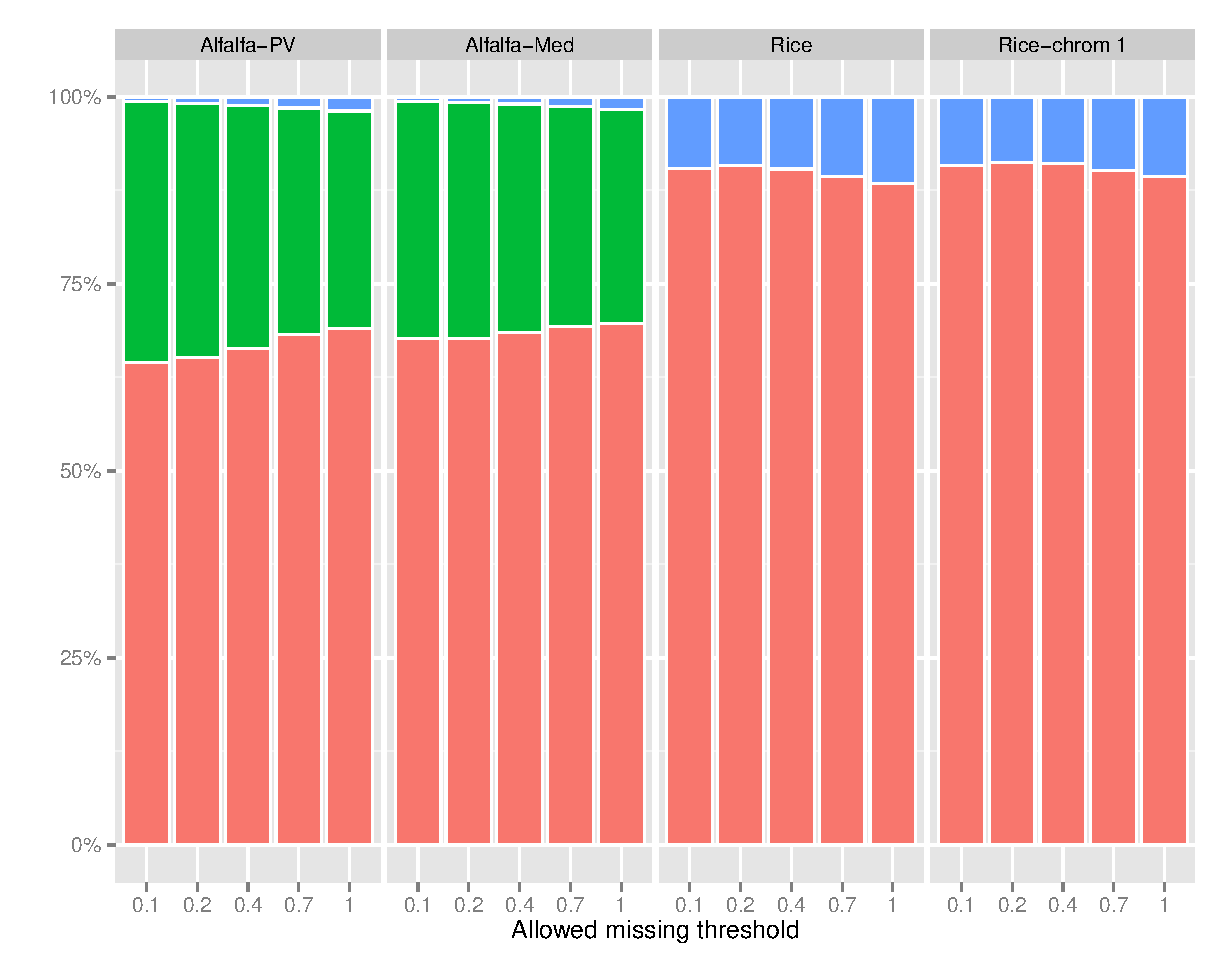
\includegraphics[width=0.95\textwidth]{Fig01_class_breakdown_all.pdf}
\caption[Proportions of genotype classes]{​Proportion of genotype classes for the different missing rate thresholds (0.1, 0.2, 0.4, 0.7 and 1 -the complete dataset), in Alfalfa-PV, Alfalfa-Med and Rice (all chromosomes and chromosome 1 only). Red bars represents the most common homozygous (AA), blue bars the least common homozygous (BB) and green bars the heterozygous (AB).}
\label{fig:genotype_classes}
\end{figure}

\subsection{Imputation accuracy}
\label{sec:imputation_accuracy}  
\textcolor{red}{
\begin{itemize}
  \item all rice chromosome gave the same results, as in Suppl figures
  \item all numbers in this section need to be checked
  \item what about supplementary figures? still valid?
\end{itemize}
}
In rice, the average imputation accuracy over all genotypic classes was above 80\% for all methods. No significant difference was found between chromosomes. Thus average accuracy over all chromosomes is therefore presented (Figure~\ref{fig:accuracy_rice}). \\
The overall accuracy for alfalfa, averaged across the two datasets, was 12-25\% lower than rice, ranging between 66\% and 84\%. No significant difference were found between the two datasets. Thus average accuracy over the Alfalfa-Med and Alfalfa-PV is presented (Figure~\ref{fig:accuracy_alfalfa}).

The imputation accuracy varied across the different genotype classes, with the highest accuracy in the most common genotype class (averaging \textcolor{red}{XXX}\% and \textcolor{red}{XXX}\% in alfalfa and rice, respectively), while the least common genotype class showed much lower accuracy (averaging \textcolor{red}{XXX}\% and \textcolor{red}{XXX}\% in alfalfa and rice, respectively).
Alfalfa datasets included heterozygous SNP loci, accounting for an average of 30\% of individuals per locus (Table~\ref{tab:descriptive_statistics}). Heterozygotes had an intermediate imputation accuracy ranging from 0\% with MNI to 70\% with KNNI. Results for each individual alfalfa population and the 12 individual rice chromosomes are similar to those discussed here (see Supplementary Figures S2 to S16). \\
Missing data did not affect the imputation accuracy substantially, with most algorithms showing a flat or almost flat response to increased missing rate. KNNI showed a decreasing imputation accuracy with increasing missing data, both in alfalfa and rice.

Beagle outperformed all other imputation methods in rice, making efficient use of marker position (Figure~\ref{fig:accuracy_rice}). When markers were randomly reshuffled (thus offsetting position information), though, general imputation methods (other than MNI) showed a higher imputation accuracy than Beagle. The accuracy loss with shuffled markers is exacerbated in alfalfa datasets, and in particular on heterozygous and minor homozygous classes.\\
Similarly, FILLIN resulted in a 5-10\% accuracy drop when marker positions were shuffled. FILLIN performances were in general lower than other methods due to the fraction of unimputed genotypes, here accounted as wrong imputation. FILLIN did not impute an average of 14.6\% missing data in Rice and practically the entirety of Alfalfa data. Even trying to relax FILLIN constraint parameters, it was impossible to obtain sensible results. Thus, FILLIN accuracy does not appear in Figure~\ref{fig:accuracy_alfalfa}.

When examining general imputation methods, resulting accuracies highlighted RFI and KNNI as the best ones. The two methods had comparable performances, without a preferable option over all experiments. SVDI followed, and MNI ranked last.\\
In Rice, for 70\% allowed missing rate datasets, the imputation accuracy of RFI was still greater than 90\%, while it dropped towards 75\% for KNNI and SVDI. As expected, MNI had an imputation accuracy of 100\% in the major homozygous class, but dropped to 0\% in the minor homozygous class.\\
In alfalfa KNNI showed the highest imputation accuracy over all classes \textcolor{red}{(XXX\%)} and in the heterozygous \textcolor{red}{(XXX\%)} and minor homozygous \textcolor{red}{(XXX\%)} genotype classes (Figure~\ref{fig:accuracy_alfalfa}). RFI and SVDI were second ranking. They did not differ much from MNI in the overall accuracy \textcolor{red}{(XXX\%)} and in the major \textcolor{red}{(XXX\%)} homozygous class, but gave higher imputation accuracy in the heterozygous \textcolor{red}{(XXX\%)} and minor homozygous \textcolor{red}{(XXX\%)} classes. 

\begin{figure}
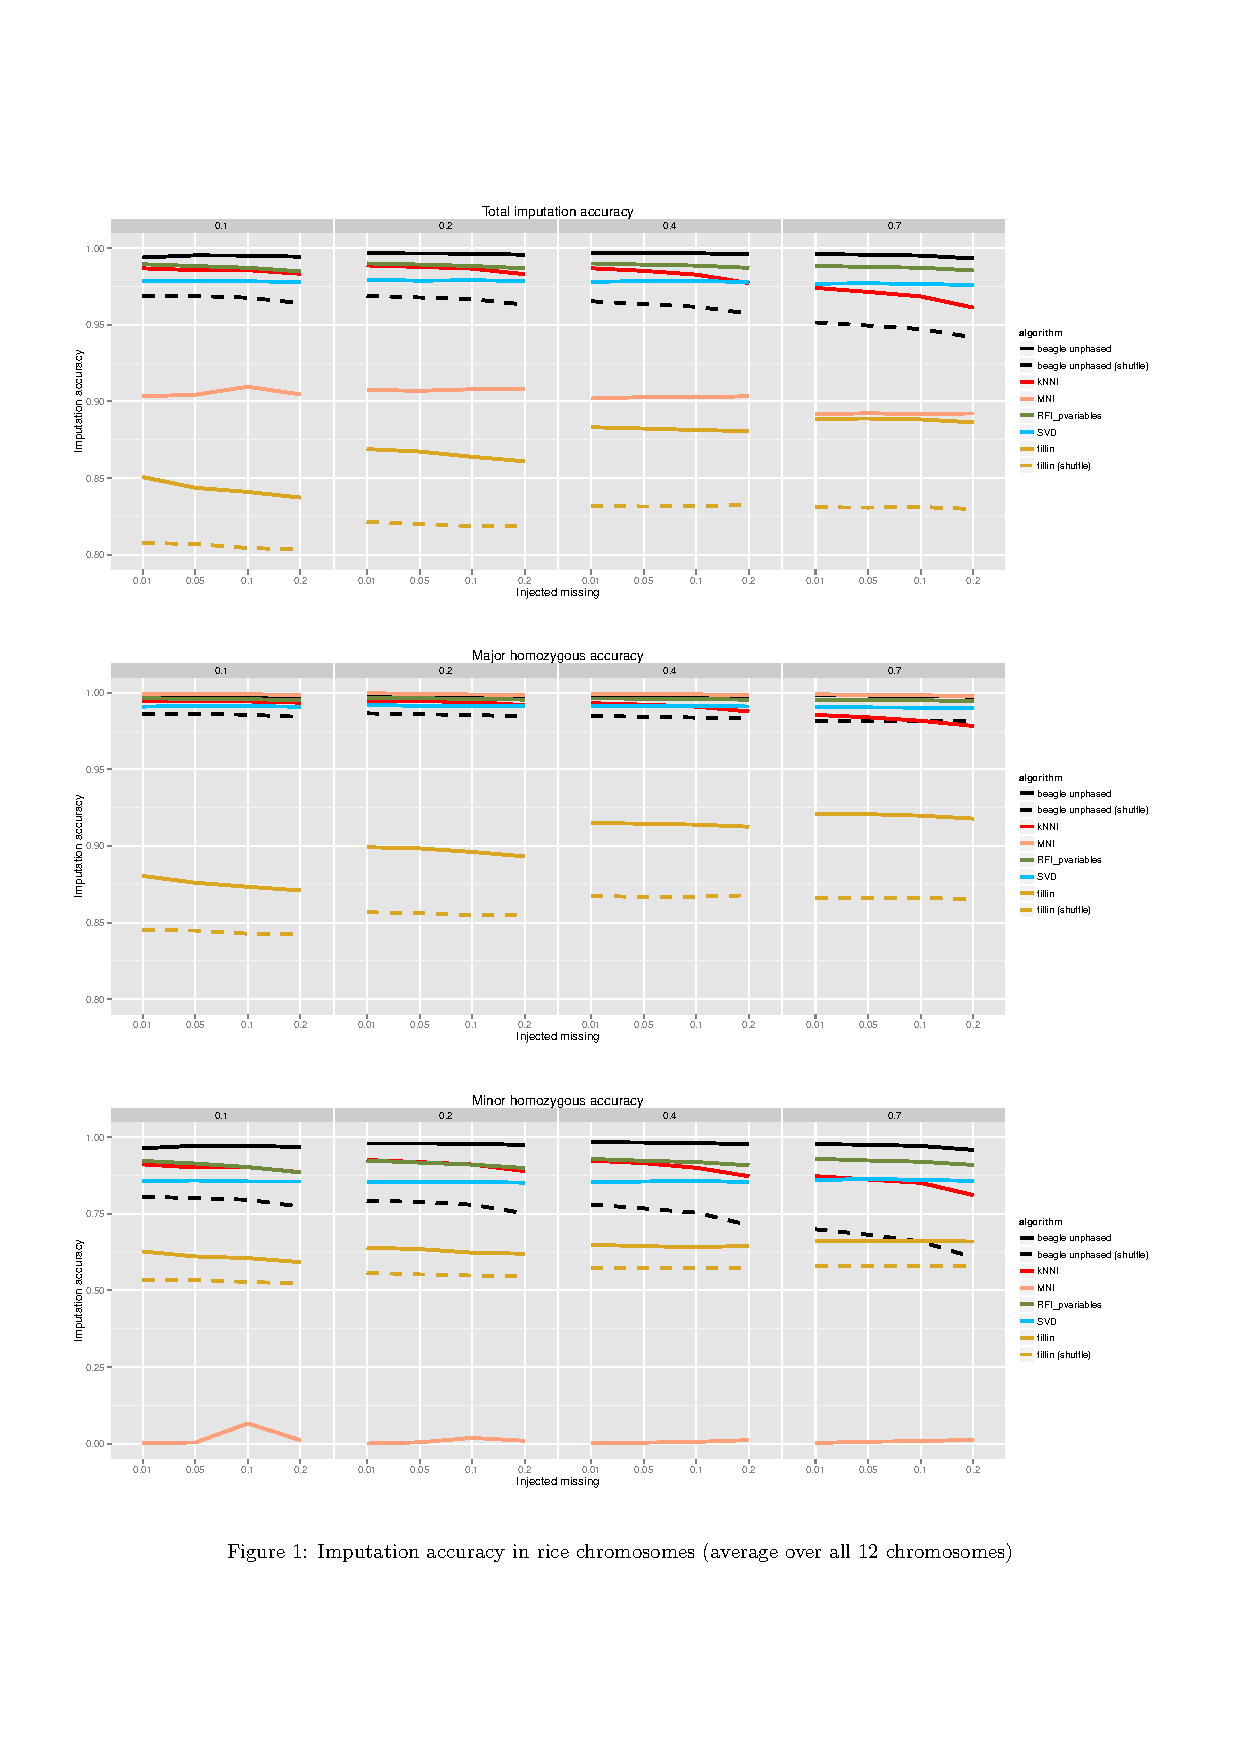
\includegraphics[width=0.95\textwidth]{figure_rice_chrom.pdf}
\caption[Rice imputation accuracies]{
imputation accuracies overall, for the major homozygous genotype (AA), and for the minor homozygous genotype (BB) in datasets consisting of 10\%, 20\%, 40\% and 70\% allowed missing data per locus (boxes) with 1\%, 5\%, 10\% and 20\% additional missing values artificially introduced (x-axis) averaged over the 12 rice chromosomes. Lines colors represent the five imputation algorithms: MNI (salmon), KNNI (red), SVDI (blue), RFI (green), Beagle with ordered markers (solid black), Beagle with unordered markers (dashed black), FILLIN with ordered markers (purple) and FILLIN with unordered markers (dashed purple). Y axis scale changes to highlight differences.}
\label{fig:accuracy_rice}
\end{figure}

\begin{figure}
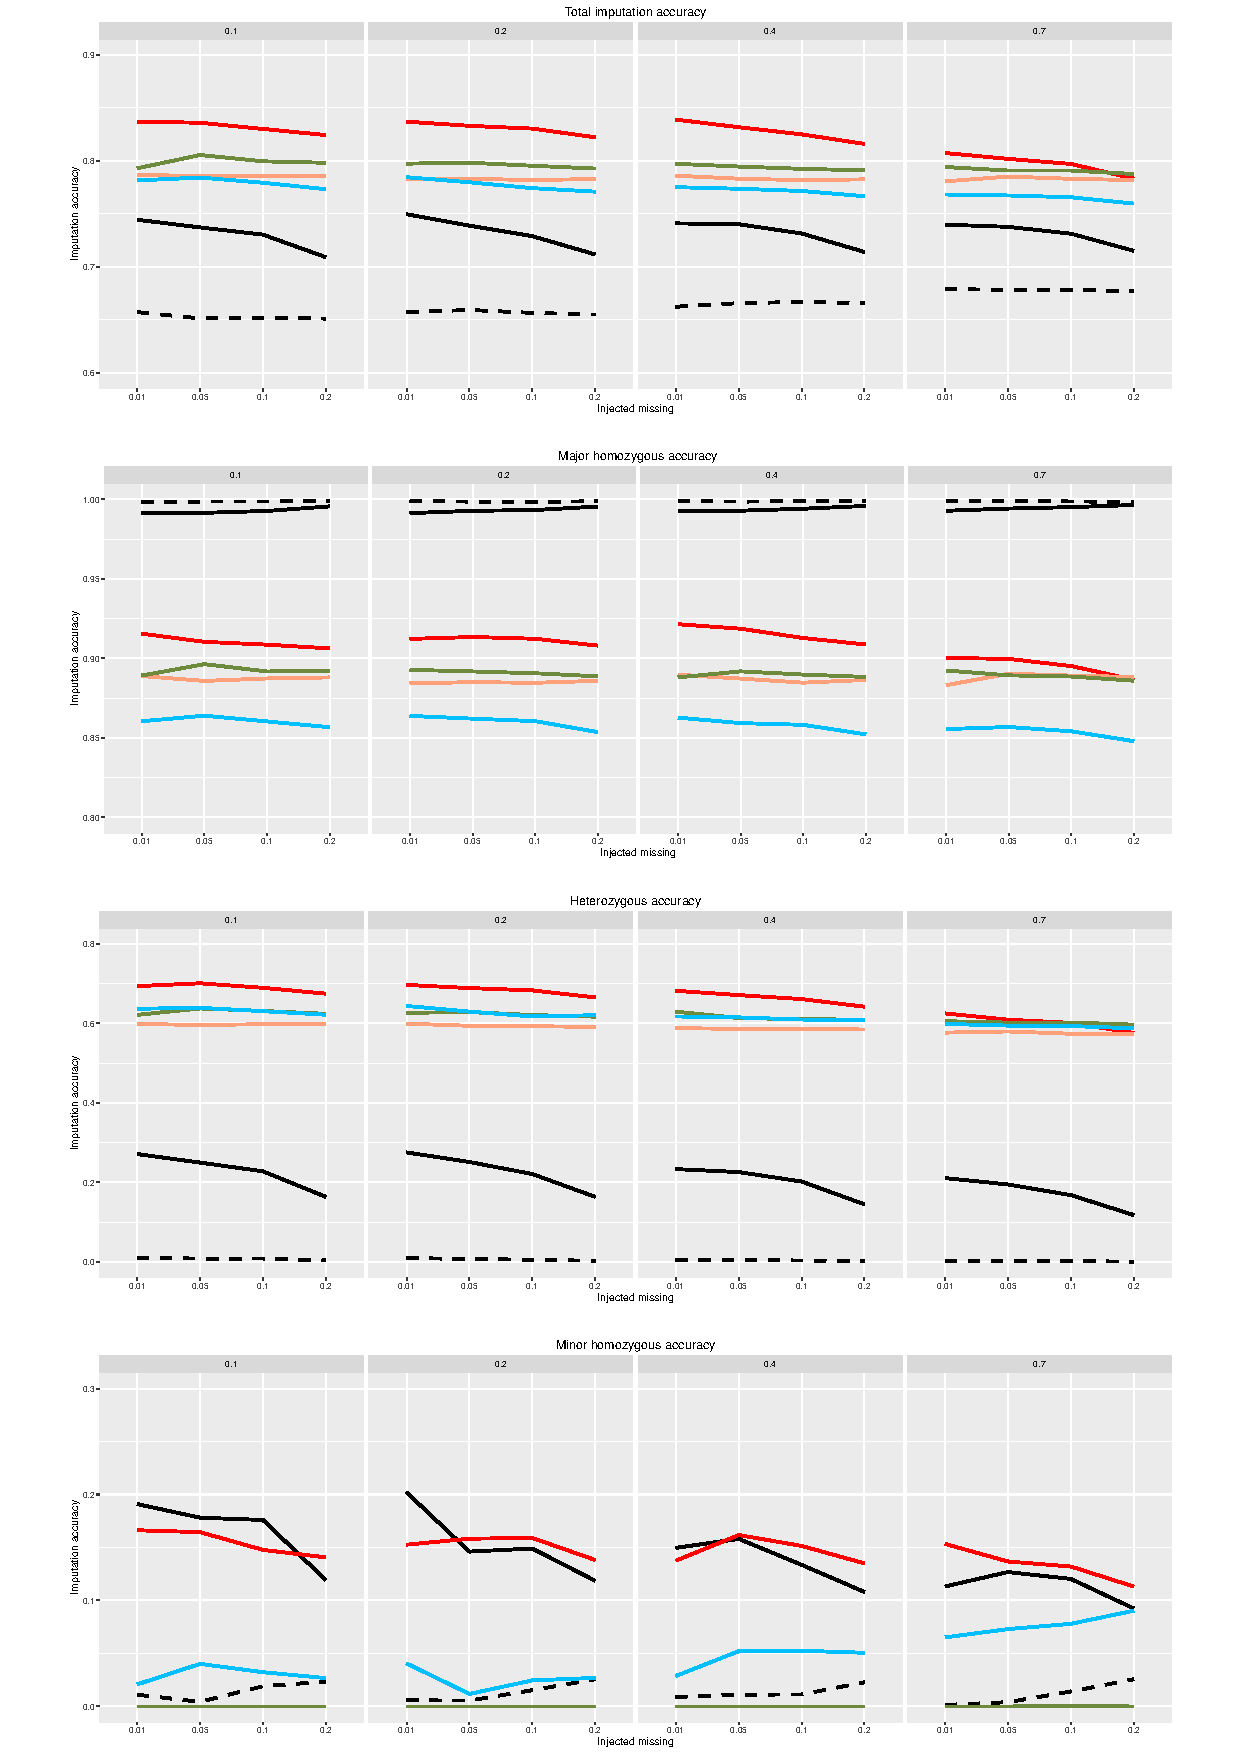
\includegraphics[width=0.95\textwidth]{figure_alfalfa.pdf}
\caption[Alfalfa imputation accuracies]{
imputation accuracies overall, for the major homozygous genotype (AA), for heterozygotes (AB), and for the minor homozygous genotype (BB) in datasets consisting of 10\%, 20\%, 40\% and 70\% allowed missing data per locus (boxes) with 1\%, 5\%, 10\% and 20\% additional missing values artificially introduced (x-axis) averaged two alfalfa populations (Alfalfa-Med and Alfalfa-PV). Lines colors represent the five imputation algorithms: MNI (salmon), KNNI (red), SVDI (blue), RFI (green), Beagle with ordered markers (solid black) and Beagle with unordered markers (dashed black). FILLIN was unable to impute alfalfa data and is absent from figure. Y axis scale changes to highlight differences.}
\label{fig:accuracy_alfalfa}
\end{figure}

\subsection{Computation time}
\label{sec:computation_time}  
The amount of time required to complete the imputation process was recorded for each method. Only the implementation of RFI could leverage a multi-core/multi-thread environment, so that RFI computation times should be evaluated considering 10 CPUs used in parallel, while all other algorithms used only one CPU at a time.\\
Imputation efficiency (Figure~\ref{fig:time_analysis}) was assessed with respect to the gross dimension of the data set (i.e., number of markers $\times$ number of samples). An alternative analysis relating computation times to the number of missing genotypes brought to the same results (data not shown).\\
RFI required by far the longest computation times (in spite of parallelization), which grew approximately exponentially ($O(e^N)$) with problem size, and easily required tens of hours for individual rice chromosomes, and hundred of hours (up to 937 hours) for the complete rice dataset. The second slowest algorithm was KNNI, with computation times growing approximately quadratically ($O(N^2)$) with problem complexity (the chosen KNNI implementation contains no heuristic method to prune the all vs. all distance calculation). KNNI was however significantly faster than RFI (on average 16.7 times faster), requiring a time ranging from 20.68 seconds (rice chromosome 7, 10\% allowed, 1\% artificial) to about 28 hours (rice complete dataset, 70\% allowed, 20\% artificial) to complete the imputation task.\\
All other algorithms were faster, with computation times growing linearly or logarithmically with problem size. Beagle, FILLIN and SVDI resulted in similar execution times. MNI was by far the fastest imputation algorithm, being scarcely affected by the size of the problem (computation times ranging from 0.23 to 31.29 seconds).

\begin{figure}
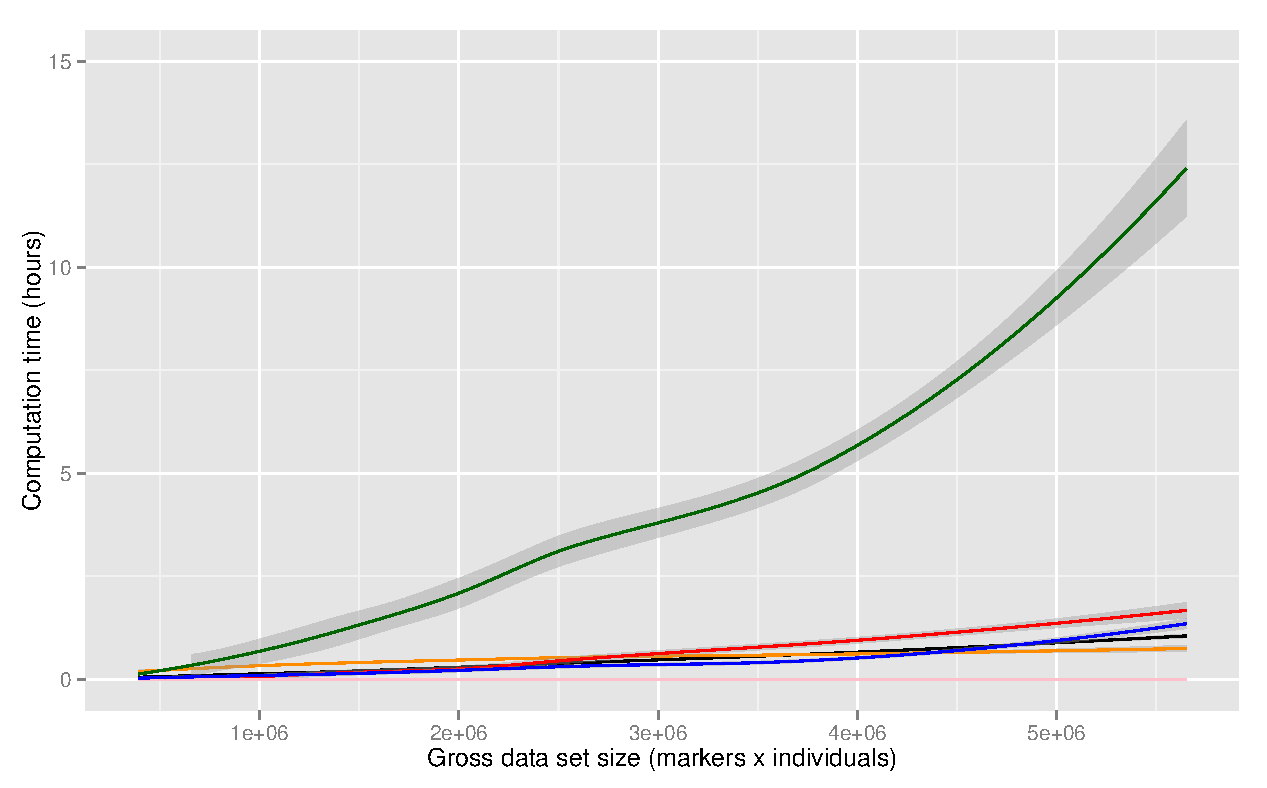
\includegraphics[width=0.95\textwidth]{time_vs_size.pdf}
\caption[Computation times]{computation time as a function of the total size of the imputed dataset.
Lines colors represent the five imputation algorithms: MNI (salmon), KNNI (red), SVDI (light blue), RFI (green), Beagle (black) and FILLIN (purple).
Plots include measures on Alfalfa-Med population, Alfalfa-PV population, and rice chromosomes 1 to 12. Complete rice datasets are omitted for readibility.}
\label{fig:time_analysis}
\end{figure}

\section{Discussion}
\label{sec:discussion}

\subsection{Minor Allele Frequency and data (un)balancedness}
\label{sec:maf}
GBS data pose a greater challenge than SNP-array data to imputation algorithms, mainly as a consequence of the much larger quantity of missing genotypes they contain. On our data sets we found missing rates varied from 53\% to 67\%. With larger amounts of missing data the complexity of the imputation problem increases. Imputation error can have a negative impact on successive analyses (see for instance \cite{rutkoski_imputation_2013,Annicchiarico2015}).\\
The imputation of missing SNP genotypes is a special case of the broader family of classification problems: three-class missing genotypes (AA, AB and BB) at any given SNP locus are classified based on known genotypes at all remaining data points. Classification problems are known to be harder when data are unbalanced, i.e. the classes appear at different frequencies in the datasets, with typically one over-represented class
(see~\cite{kotsiantis_handling_2006}
and~\cite{sun_classification_2009} for a review). In SNP genotype imputation, data balancedness is directly related to the minor allele frequency (MAF). In the classification of unbalanced observations, it is important to look not only at the total classification accuracy, but also at the per-class accuracy. The total classification accuracy may be misleading, being ``dominated'' by the majority class
\cite{he_learning_2009}.
Indeed, we found that for most methods, even when the total classification accuracy was very high, relatively large error rates were present on minority classes. 
The dependency of imputation results on MAF has already been acknowledged  (e.g.,~\cite{hickey_factors_2012} in maize; \cite{ma_comparison_2013} in cattle; \cite{pei_analyses_2008} in humans). Our per-class dissection of results allowed a deeper insight into the imputation process. Indeed, all imputation algorithms performed considerably better in the majority class rather than in the less frequent classes.
In alfalfa, KNNI was easily the best imputation method in the heterozygous and minor homozygous classes, while SVDI and RFI performed only slightly better than MNI. In rice, Beagle gave the best imputation results, with accuracy close to 100\% both in the major and minor homozygous classes. MNI performed reasonably well in the alfalfa heterozygous class, with accuracy close 60\%, contributed to its moderately good results (total accuracy around 80\%).

\subsection{Missing rate and the ``curse of dimensionality''}
\label{sec:missing_rate_curse_dimensionality}
In general, imputation methods were relatively robust to increasing missing rates. Only KNNI, and to a lesser extent RFI, showed slowly degrading performances at very high missing rates. The divergent response of the different imputation methods to missing rate became apparent only in the most challenging scenarios, when markers with up to 40-70\% missing genotypes were allowed in the data set.\\
KNNI's decrease in imputation accuracy with increasing missing rates can be interpreted in relation to the phenomenon known as the ``curse of dimensionality'' \cite{bellman_dynamic_1957,marimont_nearest_1979}: with the same amount of data, the increasing number of parameters - the ``dimensions'' of the problem - increases and complicates the identification of k neighbors which are close enough to the data point to be classified/imputed. 
On average, the side $l$ of the hypercube to include $k$ neighbors is a function of $k$, $n$ (sample size) and $p$ (number of parameters): $l = \left ( \frac{k}{n} \right )^{1/p}$. With $n$ constant, the hypercube in which the $k$ neighbors lie gets bigger as $p$ increases. This holds especially for local learning methods (e.g.,~K-Nearest Neighbors methods, local regression) which rely heavily on the the information content of the neighbourhood. RFI - which only partially relies on local structure of the data - suffered marginally from high missingness. SVD and MNI, which build on more general properties of the data, and Beagle - whose learning process is fundamentally different and specific for genotype imputation - were scarcely affected by missing rates.

\subsection{Imputation efficiency: differences in rice vs. alfalfa}
\label{sec:role_of_species}
Imputation results were significantly different in rice and alfalfa: all imputation algorithms performed consistently better in rice data sets, where Beagle, RFI and KNNI achieved performances comparable to what is reported in literature for SNP-chip data (e.g.,~\cite{vanraden_genomic_2013} for bovine data;
\cite{the_1000_genomes_project_consortium_integrated_2012}
for human data). On the other hand, imputation accuracy in alfalfa data sets was much lower. This can be ascribed to four main factors: \\
i) the imputation problem was simpler in rice than in alfalfa, as the rice dataset comprised only pure lines, i.e. only two genotype classes instead of alfalfa's three; \\
ii) the genome structure was simpler in rice (diploid) than alfalfa (autotetraploid, rendered diploid ``in silico'' during SNP calling);\\
iii) alfalfa datasets did not contain population structure \cite{Annicchiarico2015}, while rice population was intrinsically stratified - being a collection of five subpopulation. Population structure is implicitly used by algorithms as Beagle and KNNI that create clusters of similar genotypes. Thus, rice dataset population structure facilitated the inputation process;\\
iv) rice data were analyzed by chromosome, allowing for higher average values of linkage disequilibrium (LD) among SNP markers, thus simplifying the imputation process.\\
Finally, the further difference in imputation accuracy between Alfalfa-Med and Alfalfa-PV suggests that other factors, directly connected to GBS protocols, may influence the general quality of the resulting data.\\
The most dramatic difference between data sets was found in FILLIN performances. The algorithm costantly produced 100\% uninputed results in alfalfa, while resulted in average performances in rice (albeit inferior to the other algorithms). This behaviour is probably due to FILLIN being designed to target inbred lines (as the name itself indicates).

\subsection{Reference genome assembly and ordered vs unordered markers}
\label{sec:reference_genome_ordered_vs_unordered}
When a reference genome is available, markers positions can be used in the imputation process. All methods specifically developed for the imputation of missing genotypes have been designed for markers ordered along the genome sequence, and make explicit or implicit use of position information.

For alfalfa there is no reference genome sequenced yet. The genome of the close relative diploid \emph{Medicago Truncatula} is available \cite{young_medicago_2011} and could in principle be used. However, while the two genomes show high synteny \cite{li_saturated_2014}, aligning the SNPs on a genome of a different species (and with a different ploidity) would introduce a further level of complexity, and the effect of alignments errors would be hardly assessable. Moreover, the non-aligning SNPs would be discarded, not on the basis of data quality, but of local synteny. We therefore decided to not use the genome of \emph{M. Truncatula} in the present analysis.

In rice, where a reference genome is available, we could assess the effect of using ordered vs. unordered markers for imputation. Among the imputation methods used in this study, Beagle is the only one to make use of marker information, and was therefore tested with ordered and randomly reshuffled markers. Interestingly, with ordered markers Beagle shows astounding resilience to high missingness, with imputation accuracy in the minority class $>$ 0.95 even in the most extreme scenarios (70\% allowed, 20\% artificial missing genotypes).

Beagle worked substantially worse when the marker position was randomly reshuffled, with imputation accuracy in the minority class ranging from 0.75 (10\% allowed, 1\% artificial missing rates) to almost 0.5 (70\% allowed, 20\% artificial missing rates). When tested with alfalfa (with no marker position available) Beagle largerly overestimated by the majority class, performing poorly
This result confirmed that imputation methods specifically designed for ordered markers are not an option for species lacking a reference genome.

Previous studies, though not detailing a per-class breakdown of the imputation accuracy, provided interesting comparisons. In sugar beet, Biscarini et al.~\cite{biscarini_genome-enabled_2014} used Beagle to impute SNP-chip markers with partial within-chromosome/scaffold alignment, finding global accuracies ranging from 84\% to 80.9\% with 1\% to 20\% missing genotypes. Huang et al.~\cite{huang_efficient_2014} tested several algorithms, including Beagle, on simulated ordered GBS rice data with missing rates in the 30-60\% range and finding Beagle gave imputation accuracy consistently higher (+15-20\%) than KNNI. 
Finally, Swarts et al.~\cite{swarts_novel_2014} used ordered GBS maize data to compare Beagle with the FSFHap and FILLIN algorithms they developed. All these algorithms rely on a Hidden Markov Model (HMM) to detect recombination break-points between haplotypes. They mostly obtained high imputation accuracies in the three genotype classes, providing further evidence of the added value of having a reference genome assembly.

\subsection{Size of the imputation problem}
\label{sec:size_of_problem}
Albeit this was not the main objective of the paper, and no formal effort to optimise the implementation of the various imputation methods was done, still the recorded computation times give us some interesting information.
The size of the problem, besides affecting the accuracy achievable by some imputation methods, is mainly relevant with reference to the required computation resources. RFI was the most demanding algorithm, with computation times growing exponentially both with the total number of marker genotypes (m SNP $\times$ n samples) and with the number of missing genotypes to be imputed. When analyzing the complete rice dataset (all chromosomes together), RFI took a maximum of about 40 days to complete imputation, and became computationally intractable (on the available platform) for the largest missing rate scenarios. This was partially mitigated by parallelization (we used 10 CPUs in our experiments). All other imputation algorithms took much shorter times to complete imputation, even in the most challenging scenarios. Putting together imputation accuracy and computation time, we found that the best performing imputation algorithms were Beagle in rice and KNNI in alfalfa.

\section{Conclusions}
\label{sec:conclusions}
Imputation of missing genotypes can be an effective technique also for GBS data.
The most accurate imputation methods resulted in a total amount of wrongly imputed genotypes near to zero in rice and slightly over 10\% in alfalfa. 
The proportion of imputation errors, however, varied dramatically among genotype classes, approaching very high levels with the worst methods on the minor homozygous class.
The structure of the genome and the maturity of the reference assembly play a role in the imputation efficiency, as indicated by the greater efficiency obtained in rice compared with alfalfa and, most importantly, affected the relative efficiency of the methods. While Beagle was preferable for rice, general data imputation methods performed significantly better in the absence of a reference genome, such as in alfalfa. In particular, RFI and KNNI showed the lowest imputation errors in all classes, with KNNI to be preferred for computational efficiency.
The imputation accuracy tended to be relatively robust over increasing missing rates. However, KNNI showed a somewhat lower accuracy on high missingness scenarios, probably as a consequence of the ``curse of dimensionality''. In terms of computation requirements, all methods proved to be tractable over all problem complexities with a standard bioinformatics-lab computation infrastructure, except RFI (whose computational requirements increased exponentially with problem size and took up to 40 days with the complete rice dataset and maximum missing rate thresholds).\\
Exploring ways to improve imputation accuracy in GBS data, for instance by combining predictive methods as in boosting or model ensembling, while at the same time increasing algorithm efficiency to keep computation times reasonably low, is an important research area, and can help making low-cost genotyping-by-sequencing a very cost-effective technique for genomic applications in species with and without a reference genome.


\begin{acknowledgements}
The rice data used in this research paper were produced within the framework of the Italian national project ``RISINNOVA'' (grant n. 2010-2369), financially supported by the AGER Foundation..
The creation of the alfalfa data sets was funded by the projects ‘Genomic selection in alfalfa (GENALFA)’ funded by the Italian Ministry of Foreign Affairs and International Cooperation in the framework of the Italy-USA scientific cooperation program, the Italian share of the FP7-ArimNet project ‘Resilient, water- and energy-efficient forage and feed crops for Mediterranean agricultural systems (REFORMA)’ funded by the Italian Ministry of Agricultural and Forestry Policies.
\end{acknowledgements}




% BibTeX users please use one of
%\bibliographystyle{spbasic}      % basic style, author-year citations
\bibliographystyle{spmpsci}      % mathematics and physical sciences
%\bibliographystyle{spphys}       % APS-like style for physics
\bibliography{inputs/nazzicari.bib}   % name your BibTeX data base


\end{document}
% end of file template.tex

